% Options for packages loaded elsewhere
% Options for packages loaded elsewhere
\PassOptionsToPackage{unicode}{hyperref}
\PassOptionsToPackage{hyphens}{url}
\PassOptionsToPackage{dvipsnames,svgnames,x11names}{xcolor}
%
\documentclass[
  11pt,
  letterpaper,
]{article}
\usepackage{xcolor}
\usepackage[margin=1in,headheight=14pt]{geometry}
\usepackage{amsmath,amssymb}
\setcounter{secnumdepth}{-\maxdimen} % remove section numbering
\usepackage{iftex}
\ifPDFTeX
  \usepackage[T1]{fontenc}
  \usepackage[utf8]{inputenc}
  \usepackage{textcomp} % provide euro and other symbols
\else % if luatex or xetex
  \usepackage{unicode-math} % this also loads fontspec
  \defaultfontfeatures{Scale=MatchLowercase}
  \defaultfontfeatures[\rmfamily]{Ligatures=TeX,Scale=1}
\fi
\usepackage{lmodern}
\ifPDFTeX\else
  % xetex/luatex font selection
\fi
% Use upquote if available, for straight quotes in verbatim environments
\IfFileExists{upquote.sty}{\usepackage{upquote}}{}
\IfFileExists{microtype.sty}{% use microtype if available
  \usepackage[]{microtype}
  \UseMicrotypeSet[protrusion]{basicmath} % disable protrusion for tt fonts
}{}
\makeatletter
\@ifundefined{KOMAClassName}{% if non-KOMA class
  \IfFileExists{parskip.sty}{%
    \usepackage{parskip}
  }{% else
    \setlength{\parindent}{0pt}
    \setlength{\parskip}{6pt plus 2pt minus 1pt}}
}{% if KOMA class
  \KOMAoptions{parskip=half}}
\makeatother
% Make \paragraph and \subparagraph free-standing
\makeatletter
\ifx\paragraph\undefined\else
  \let\oldparagraph\paragraph
  \renewcommand{\paragraph}{
    \@ifstar
      \xxxParagraphStar
      \xxxParagraphNoStar
  }
  \newcommand{\xxxParagraphStar}[1]{\oldparagraph*{#1}\mbox{}}
  \newcommand{\xxxParagraphNoStar}[1]{\oldparagraph{#1}\mbox{}}
\fi
\ifx\subparagraph\undefined\else
  \let\oldsubparagraph\subparagraph
  \renewcommand{\subparagraph}{
    \@ifstar
      \xxxSubParagraphStar
      \xxxSubParagraphNoStar
  }
  \newcommand{\xxxSubParagraphStar}[1]{\oldsubparagraph*{#1}\mbox{}}
  \newcommand{\xxxSubParagraphNoStar}[1]{\oldsubparagraph{#1}\mbox{}}
\fi
\makeatother


\usepackage{longtable,booktabs,array}
\usepackage{calc} % for calculating minipage widths
% Correct order of tables after \paragraph or \subparagraph
\usepackage{etoolbox}
\makeatletter
\patchcmd\longtable{\par}{\if@noskipsec\mbox{}\fi\par}{}{}
\makeatother
% Allow footnotes in longtable head/foot
\IfFileExists{footnotehyper.sty}{\usepackage{footnotehyper}}{\usepackage{footnote}}
\makesavenoteenv{longtable}
\usepackage{graphicx}
\makeatletter
\newsavebox\pandoc@box
\newcommand*\pandocbounded[1]{% scales image to fit in text height/width
  \sbox\pandoc@box{#1}%
  \Gscale@div\@tempa{\textheight}{\dimexpr\ht\pandoc@box+\dp\pandoc@box\relax}%
  \Gscale@div\@tempb{\linewidth}{\wd\pandoc@box}%
  \ifdim\@tempb\p@<\@tempa\p@\let\@tempa\@tempb\fi% select the smaller of both
  \ifdim\@tempa\p@<\p@\scalebox{\@tempa}{\usebox\pandoc@box}%
  \else\usebox{\pandoc@box}%
  \fi%
}
% Set default figure placement to htbp
\def\fps@figure{htbp}
\makeatother


% definitions for citeproc citations
\NewDocumentCommand\citeproctext{}{}
\NewDocumentCommand\citeproc{mm}{%
  \begingroup\def\citeproctext{#2}\cite{#1}\endgroup}
\makeatletter
 % allow citations to break across lines
 \let\@cite@ofmt\@firstofone
 % avoid brackets around text for \cite:
 \def\@biblabel#1{}
 \def\@cite#1#2{{#1\if@tempswa , #2\fi}}
\makeatother
\newlength{\cslhangindent}
\setlength{\cslhangindent}{1.5em}
\newlength{\csllabelwidth}
\setlength{\csllabelwidth}{3em}
\newenvironment{CSLReferences}[2] % #1 hanging-indent, #2 entry-spacing
 {\begin{list}{}{%
  \setlength{\itemindent}{0pt}
  \setlength{\leftmargin}{0pt}
  \setlength{\parsep}{0pt}
  % turn on hanging indent if param 1 is 1
  \ifodd #1
   \setlength{\leftmargin}{\cslhangindent}
   \setlength{\itemindent}{-1\cslhangindent}
  \fi
  % set entry spacing
  \setlength{\itemsep}{#2\baselineskip}}}
 {\end{list}}
\usepackage{calc}
\newcommand{\CSLBlock}[1]{\hfill\break\parbox[t]{\linewidth}{\strut\ignorespaces#1\strut}}
\newcommand{\CSLLeftMargin}[1]{\parbox[t]{\csllabelwidth}{\strut#1\strut}}
\newcommand{\CSLRightInline}[1]{\parbox[t]{\linewidth - \csllabelwidth}{\strut#1\strut}}
\newcommand{\CSLIndent}[1]{\hspace{\cslhangindent}#1}



\setlength{\emergencystretch}{3em} % prevent overfull lines

\providecommand{\tightlist}{%
  \setlength{\itemsep}{0pt}\setlength{\parskip}{0pt}}



 


% hyperref-colors.tex
\usepackage{xcolor}
\usepackage{hyperref}

% Unjournal colours
\definecolor{unjournalgreen}{HTML}{99BB66}
\definecolor{unjournalorange}{HTML}{F19E4B}

\hypersetup{
  colorlinks = true,
  linkcolor  = unjournalgreen,   % internal links (TOC, sections, refs)
  citecolor  = unjournalorange,  % citations
  urlcolor   = unjournalorange   % URLs
}

% --- Compact spacing for working paper ---
\usepackage{titlesec}
\titlespacing*{\section}{0pt}{1.5ex plus 0.5ex minus 0.2ex}{0.8ex plus 0.2ex}
\titlespacing*{\subsection}{0pt}{1.2ex plus 0.3ex minus 0.2ex}{0.5ex plus 0.1ex}
\usepackage{booktabs}
\usepackage{longtable}
\usepackage{array}
\usepackage{multirow}
\usepackage{wrapfig}
\usepackage{float}
\usepackage{colortbl}
\usepackage{pdflscape}
\usepackage{tabu}
\usepackage{threeparttable}
\usepackage{threeparttablex}
\usepackage[normalem]{ulem}
\usepackage{makecell}
\usepackage{xcolor}
\makeatletter
\@ifpackageloaded{tcolorbox}{}{\usepackage[skins,breakable]{tcolorbox}}
\@ifpackageloaded{fontawesome5}{}{\usepackage{fontawesome5}}
\definecolor{quarto-callout-color}{HTML}{909090}
\definecolor{quarto-callout-note-color}{HTML}{0758E5}
\definecolor{quarto-callout-important-color}{HTML}{CC1914}
\definecolor{quarto-callout-warning-color}{HTML}{EB9113}
\definecolor{quarto-callout-tip-color}{HTML}{00A047}
\definecolor{quarto-callout-caution-color}{HTML}{FC5300}
\definecolor{quarto-callout-color-frame}{HTML}{acacac}
\definecolor{quarto-callout-note-color-frame}{HTML}{4582ec}
\definecolor{quarto-callout-important-color-frame}{HTML}{d9534f}
\definecolor{quarto-callout-warning-color-frame}{HTML}{f0ad4e}
\definecolor{quarto-callout-tip-color-frame}{HTML}{02b875}
\definecolor{quarto-callout-caution-color-frame}{HTML}{fd7e14}
\makeatother
\makeatletter
\@ifpackageloaded{bookmark}{}{\usepackage{bookmark}}
\makeatother
\makeatletter
\@ifpackageloaded{caption}{}{\usepackage{caption}}
\AtBeginDocument{%
\ifdefined\contentsname
  \renewcommand*\contentsname{Table of contents}
\else
  \newcommand\contentsname{Table of contents}
\fi
\ifdefined\listfigurename
  \renewcommand*\listfigurename{List of Figures}
\else
  \newcommand\listfigurename{List of Figures}
\fi
\ifdefined\listtablename
  \renewcommand*\listtablename{List of Tables}
\else
  \newcommand\listtablename{List of Tables}
\fi
\ifdefined\figurename
  \renewcommand*\figurename{Figure}
\else
  \newcommand\figurename{Figure}
\fi
\ifdefined\tablename
  \renewcommand*\tablename{Table}
\else
  \newcommand\tablename{Table}
\fi
}
\@ifpackageloaded{float}{}{\usepackage{float}}
\floatstyle{ruled}
\@ifundefined{c@chapter}{\newfloat{codelisting}{h}{lop}}{\newfloat{codelisting}{h}{lop}[chapter]}
\floatname{codelisting}{Listing}
\newcommand*\listoflistings{\listof{codelisting}{List of Listings}}
\makeatother
\makeatletter
\makeatother
\makeatletter
\@ifpackageloaded{caption}{}{\usepackage{caption}}
\@ifpackageloaded{subcaption}{}{\usepackage{subcaption}}
\makeatother
\usepackage{bookmark}
\IfFileExists{xurl.sty}{\usepackage{xurl}}{} % add URL line breaks if available
\urlstyle{same}
\hypersetup{
  pdftitle={Limits of AI peer review on real expert review data},
  pdfauthor={Valentin Klotzbücher; David Reinstein; Lorenzo Pacchiardi; Tianmai Michael Zhang},
  colorlinks=true,
  linkcolor={blue},
  filecolor={Maroon},
  citecolor={Blue},
  urlcolor={Blue},
  pdfcreator={LaTeX via pandoc}}


\title{Limits of AI peer review on real expert review data}
\author{Valentin Klotzbücher \and David Reinstein \and Lorenzo
Pacchiardi \and Tianmai Michael Zhang}
\date{2026-02-18}
\begin{document}
\maketitle
\begin{abstract}
We benchmark how frontier LLMs critique, rate, and prioritize research,
comparing AI-generated evaluations to human expert assessments from The
Unjournal. Human ratings serve as a reference signal---the core goal is
measuring and diagnosing AI reasoning quality: understanding
calibration, failure modes, and systematic ``taste'' differences between
AI and human evaluators.
\end{abstract}


\bookmarksetup{startatroot}

\section{Introduction}\label{introduction}

\begin{tcolorbox}[enhanced jigsaw, opacityback=0, leftrule=.75mm, titlerule=0mm, toptitle=1mm, opacitybacktitle=0.6, colframe=quarto-callout-note-color-frame, left=2mm, arc=.35mm, coltitle=black, breakable, bottomrule=.15mm, bottomtitle=1mm, colback=white, colbacktitle=quarto-callout-note-color!10!white, toprule=.15mm, title=\textcolor{quarto-callout-note-color}{\faInfo}\hspace{0.5em}{Working paper}, rightrule=.15mm]

This is an evolving working paper. Analysis, metrics, and comparisons
are under active development.

\end{tcolorbox}

Peer review is under strain. Reviewers are hard to find, turnaround
times are lengthening, and the system costs an estimated \$1.5 billion
per year in the United States alone
(\citeproc{ref-aczel2021billion}{Aczel, Szaszi, and Holcombe 2021}). An
influx of AI-generated manuscripts is likely to intensify the bottleneck
(\citeproc{ref-eger2025}{Eger et al. 2025}). If frontier language models
could produce reliable, structured evaluations of research, they might
free substantial scientific resources and deliver faster, more detailed
feedback.

We test this possibility using \href{https://unjournal.org}{The
Unjournal's} structured human evaluations as a benchmark. We prompt six
frontier LLMs---GPT-5 Pro, GPT-5.2 Pro, GPT-4o-mini, Claude Sonnet 4,
Claude Opus 4.6, and Gemini 2.0 Flash---with the same rubric and
guidelines used by human evaluators, then compare the resulting
quantitative ratings and qualitative critiques against human evaluations
for 60 economics and social-science working papers. We ask whether
frontier AI evaluations can reliably approximate human expert judgment,
which models perform best across rating criteria and cost tiers, and
whether systematic differences reveal characteristic AI preferences over
research.

The Unjournal setting is particularly well suited for this comparison.
It commissions paid expert evaluations using a structured rubric
covering seven percentile criteria with 90\% credible intervals plus
journal-tier predictions, and publishes the resulting packages
openly---reducing classic gatekeeping motives and increasing reviewer
effort. The resulting ratings and critiques still exhibit substantial
inter-rater variation; accordingly, we treat human evaluations as a
high-quality but noisy \emph{reference signal}, not ground truth. The
rich, multi-dimensional data allow us to compare the priorities and
calibration of humans and AI models across criteria and domains, while
the journal-tier predictions provide an external reference
point\footnote{These represent verifiable publication outcomes, not
  statements about the ``true quality'' of the paper.} enabling a
human-vs-LLM horse race. Finally, The Unjournal's pipeline of future
evaluations allows for clean out-of-training-data predictions, serving
as a live testing lab for prospective validation.

A growing literature examines LLM-assisted peer review, error detection,
and AI research evaluation; we survey this work in
Section~\ref{sec-related-work}. Our approach differs from prior work by
focusing on structured, percentile-based quantitative ratings with
credible intervals, comparing against published human evaluations rather
than using LLM-as-judge, and curating contamination-aware inputs.

\textbf{Acknowledgements.}

This work is a collaboration with \href{https://unjournal.org}{The
Unjournal}, which has published 55+ detailed evaluation packages
building open, quantitative evaluation infrastructure for
global-priorities-relevant research in economics, policy, and social
science. We thank The Unjournal's evaluation community for generating
the structured human assessments that make this benchmarking possible.

Funding for The Unjournal has been provided by the Survival and
Flourishing Fund, the Long Term Future Fund, and EA Funds. Portions of
this manuscript were drafted with AI assistance and reviewed by the
authors.

\bookmarksetup{startatroot}

\section{Results}\label{results}

We evaluate 6 frontier LLMs against human expert reviews from
\href{https://unjournal.pubpub.org}{The Unjournal} for 45 papers with
both human and LLM evaluations. Each model receives the same PDF, system
prompt mirroring The Unjournal rubric, and JSON schema requiring a
diagnostic summary plus numeric midpoints and 90\% credible intervals
for every metric. Full methodological details appear in
\href{methods.qmd}{Data and Methods}.

\textbf{Per-paper overview.} Figure~\ref{fig-forest-overall} displays
individual human evaluator ratings (green circles with 90\% CIs)
alongside the GPT-5 Pro LLM rating (orange diamond with CI) for each
paper's overall score. Papers are ordered by human mean rating. Dotted
lines mark grand means.

\begin{figure}

\caption{\label{fig-forest-overall}Per-paper overall ratings: individual
human evaluators (green) vs GPT-5 Pro (orange)}

\pandocbounded{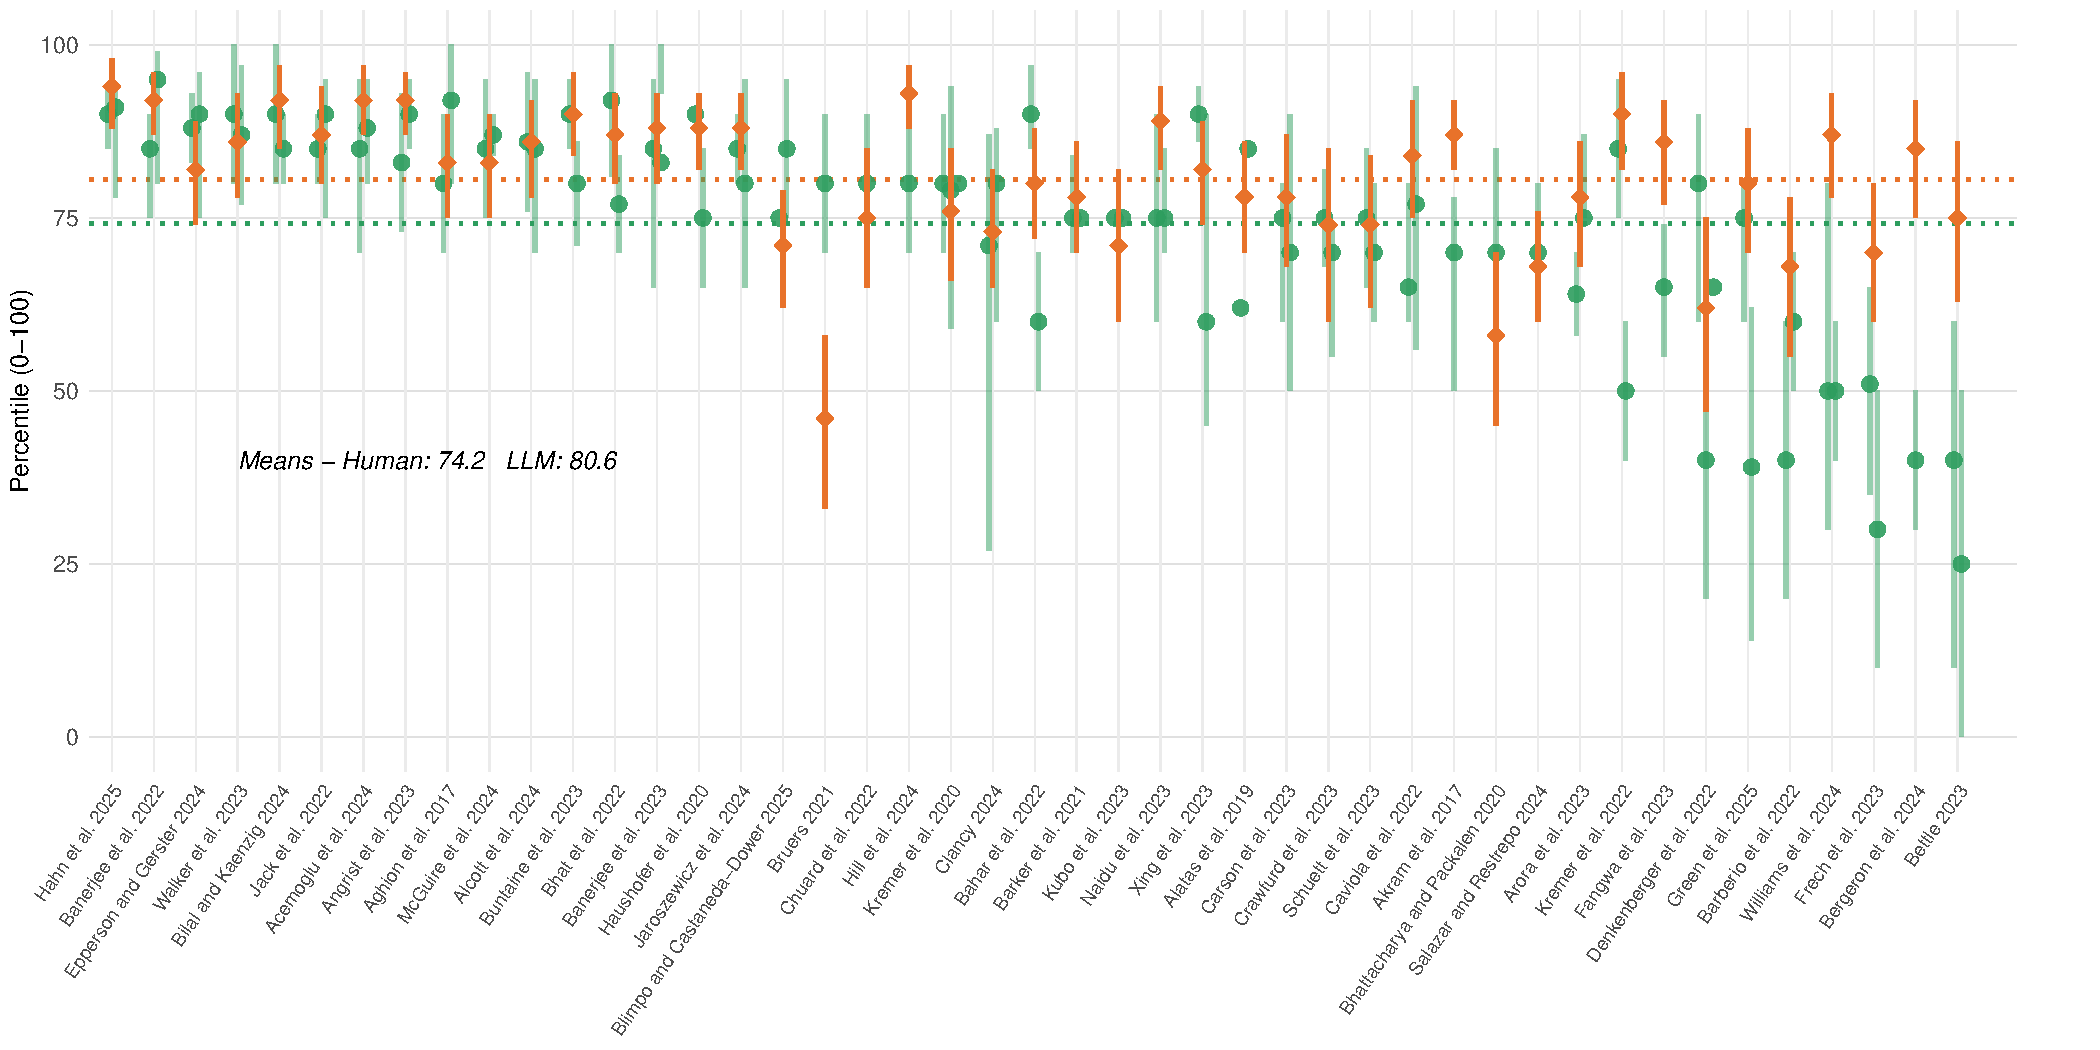
\includegraphics[keepaspectratio]{results_files/figure-pdf/fig-forest-overall-1.pdf}}

\end{figure}%

The spread of green circles within each paper column illustrates
substantial human inter-rater variability---CIs often span 20--40
points. In most cases the LLM diamond sits comfortably within the range
of human opinions, though several papers show the LLM falling outside
the human consensus.

\textbf{Overall ratings.} Figure~\ref{fig-scatter-focal} compares
overall ratings from GPT-5 Pro and Claude Opus 4.6---the two
highest-performing reasoning models---against human mean ratings. Points
on the diagonal indicate perfect agreement; distance from the line
reflects disagreement.

\begin{figure}

\caption{\label{fig-scatter-focal}Human vs LLM overall ratings: GPT-5
Pro and Claude Opus 4.6}

\pandocbounded{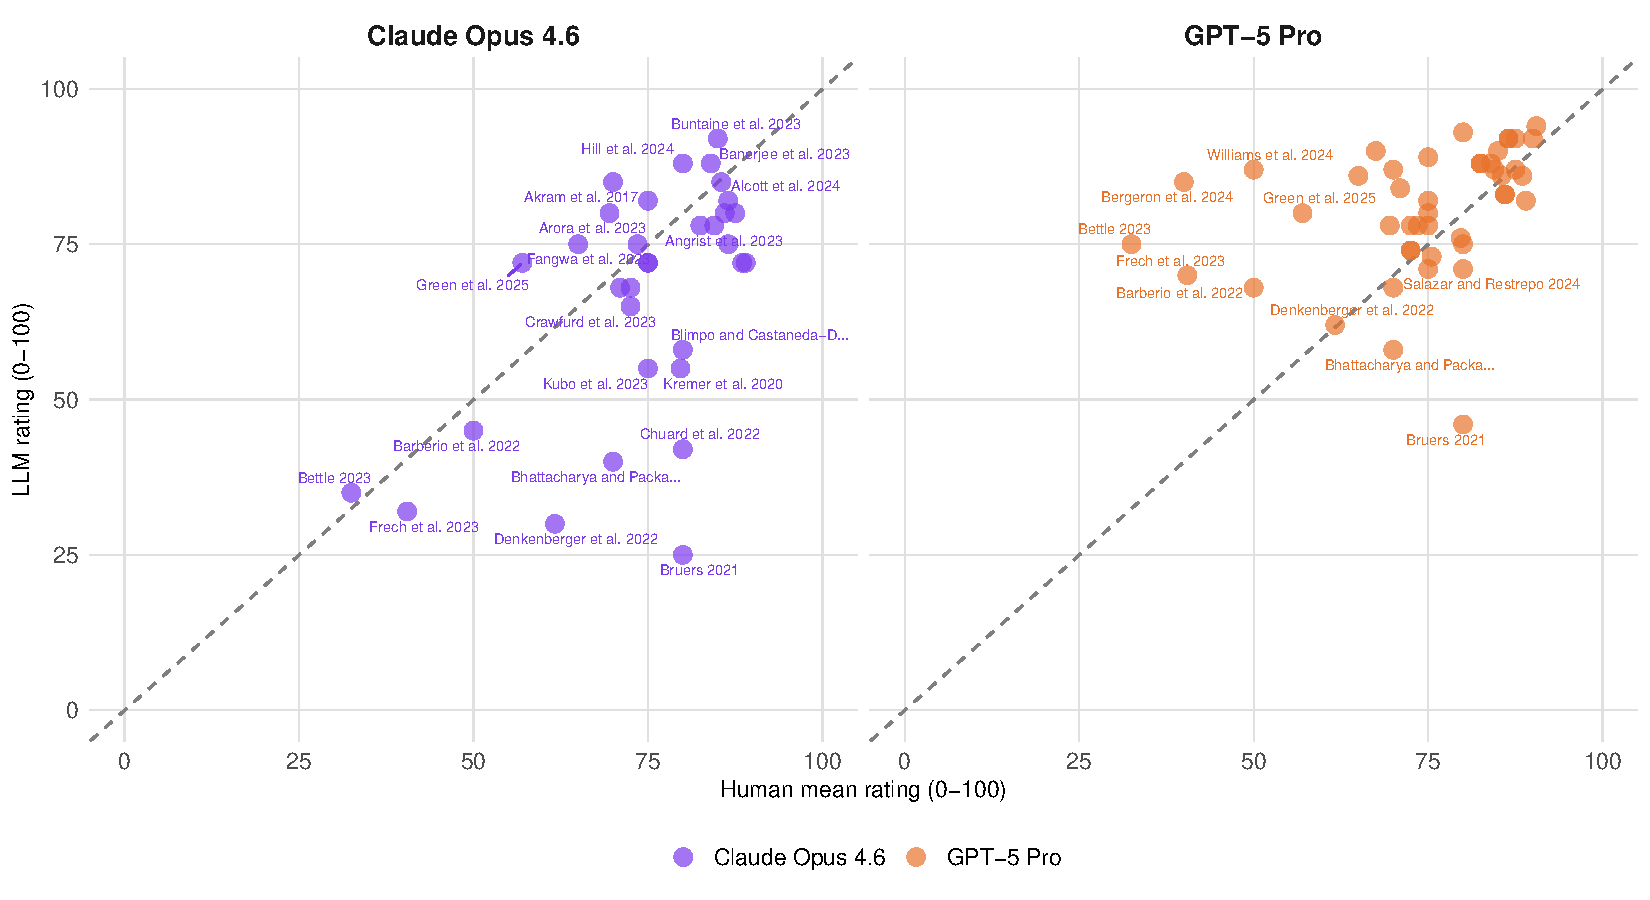
\includegraphics[keepaspectratio]{results_files/figure-pdf/fig-scatter-focal-1.pdf}}

\end{figure}%

Both models cluster around the identity line in the 40--80 range but
diverge more at the extremes. LLMs tend to compress ratings toward the
centre of the scale relative to humans, producing narrower spread---a
pattern consistent with alignment training that discourages extreme
outputs. Where humans rate a paper very highly or very harshly, the LLM
typically pulls toward the middle. Full agreement metrics including
Pearson \emph{r}, Spearman \emph{ρ}, mean bias, and RMSE for all six
models appear in Table~\ref{tbl-agreement}.

\textbf{Rank comparison.} Figure~\ref{fig-rankslope-main} contrasts the
relative \emph{ranking} of papers under human vs LLM scoring for GPT-5
Pro (left) and Claude Opus 4.6 (right). Each paper is a curve connecting
its human rank (left axis) to its LLM rank (right axis). Horizontal
lines indicate agreement; orange curves slope upward where the LLM ranks
a paper higher than humans did, and green curves slope downward where
humans rank it higher.

\begin{figure}

\caption{\label{fig-rankslope-main}Relative ranking (overall): GPT-5 Pro
(left) and Claude Opus 4.6 (right) vs Human evaluators}

\pandocbounded{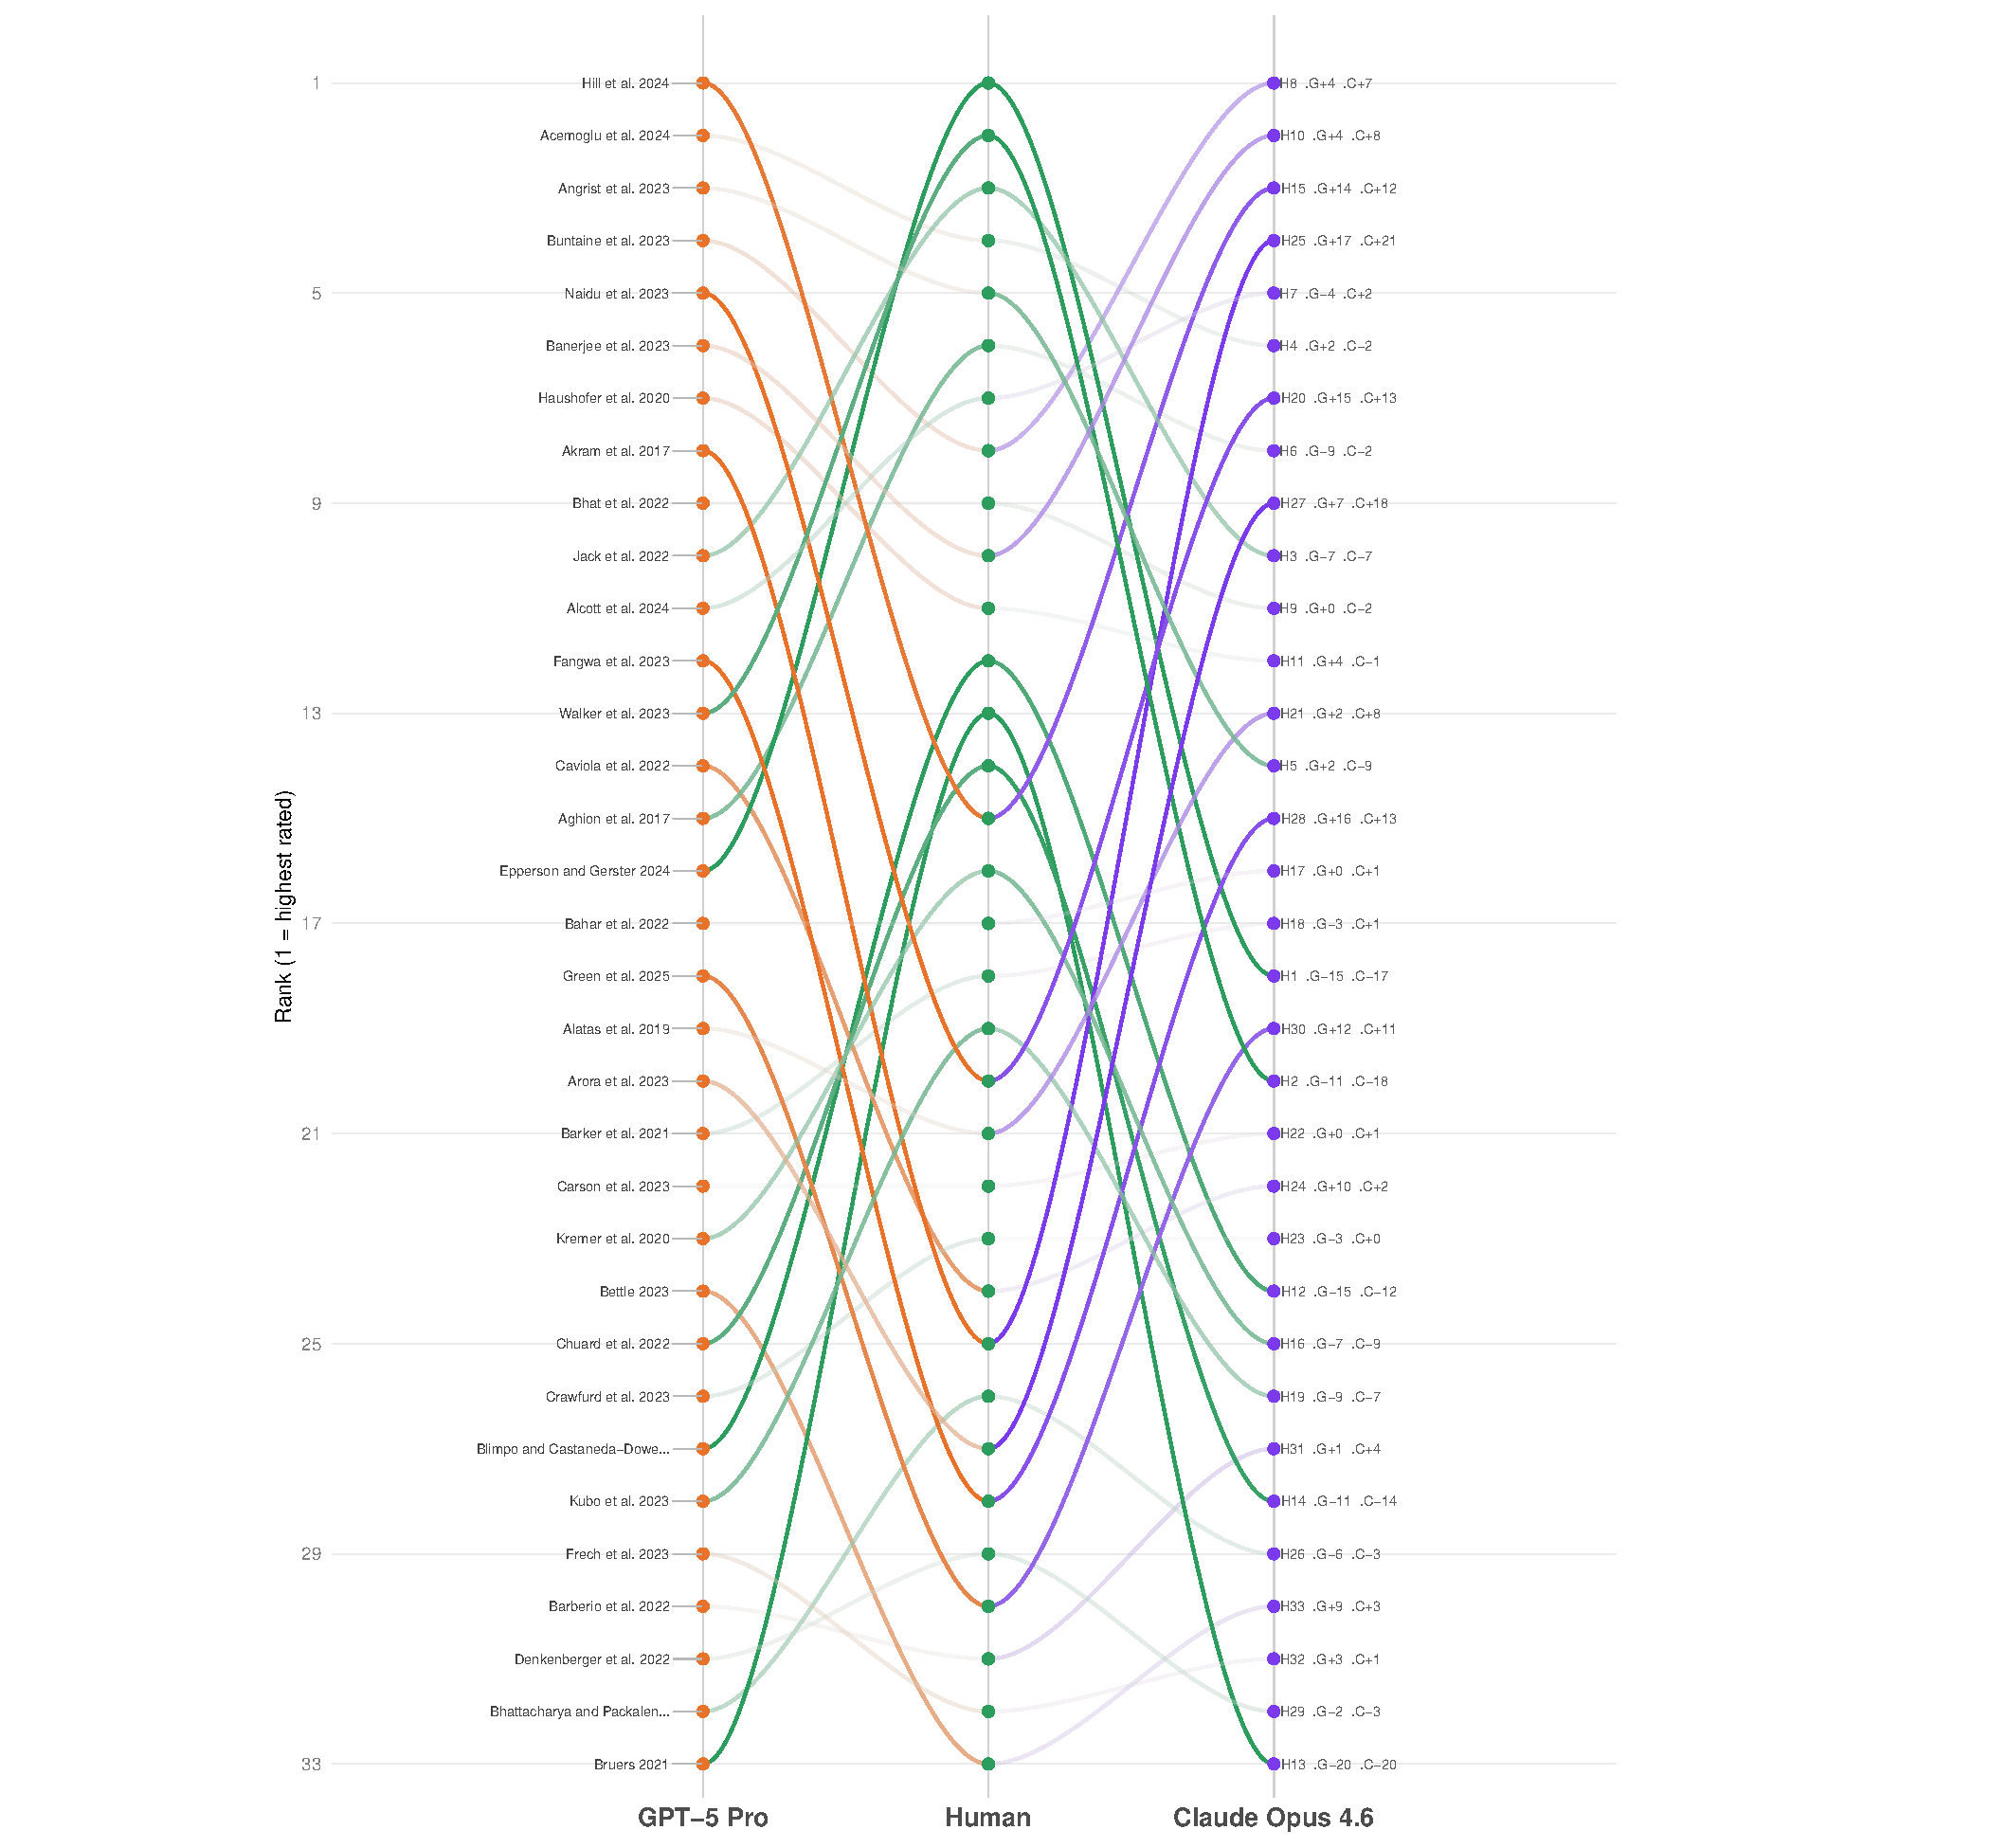
\includegraphics[keepaspectratio]{results_files/figure-pdf/fig-rankslope-main-1.pdf}}

\end{figure}%

Many papers sit close to horizontal, indicating broad agreement on
relative quality. However, several show pronounced rank shifts---orange
curves mark papers the LLM considers top-tier that humans placed lower,
while green curves highlight the reverse. Comparing the two panels
reveals whether rank disagreements are idiosyncratic to a single model
or reflect systematic ``taste'' differences shared across LLMs. The
criteria-level Krippendorff's alpha analysis in
Table~\ref{tbl-human-baseline} quantifies where human--LLM agreement
approaches the ceiling set by human inter-rater variability.

\textbf{Qualitative critique comparison.} Beyond numeric ratings, we
compare the substantive critiques each model raises against the
consensus issues identified by human experts. The figure below plots
coverage (what fraction of human concerns the LLM also identified)
against precision (what fraction of LLM-raised issues correspond to
human concerns) for each paper, as assessed by GPT-5.2 Pro acting as
judge.

Coverage and precision vary substantially across papers. Some papers
achieve high scores on both dimensions, indicating strong alignment
between human and LLM critiques, while others reveal the LLM missing key
human concerns or raising issues absent from the expert consensus. These
metrics are themselves LLM-assessed (GPT-5.2 Pro as judge); human
validation through manual annotation is underway. Detailed
paper-by-paper comparisons with matched issue pairs appear in
\href{results_critiques.qmd}{Appendix: Critiques \& Key Issues}.

\textbf{Rating differences by paper.} Figure~\ref{fig-gap-heatmap-main}
shows Human − LLM differences for each paper and criterion using GPT-5
Pro as the focal model. Green tiles indicate humans rated higher; orange
indicates the LLM rated higher. Papers are ordered by their overall
rating difference, revealing which papers drive the largest
disagreements and whether those disagreements are concentrated on
particular criteria or spread across the board.

\begin{figure}

\caption{\label{fig-gap-heatmap-main}Human − LLM rating differences by
paper and criterion (GPT-5 Pro)}

\pandocbounded{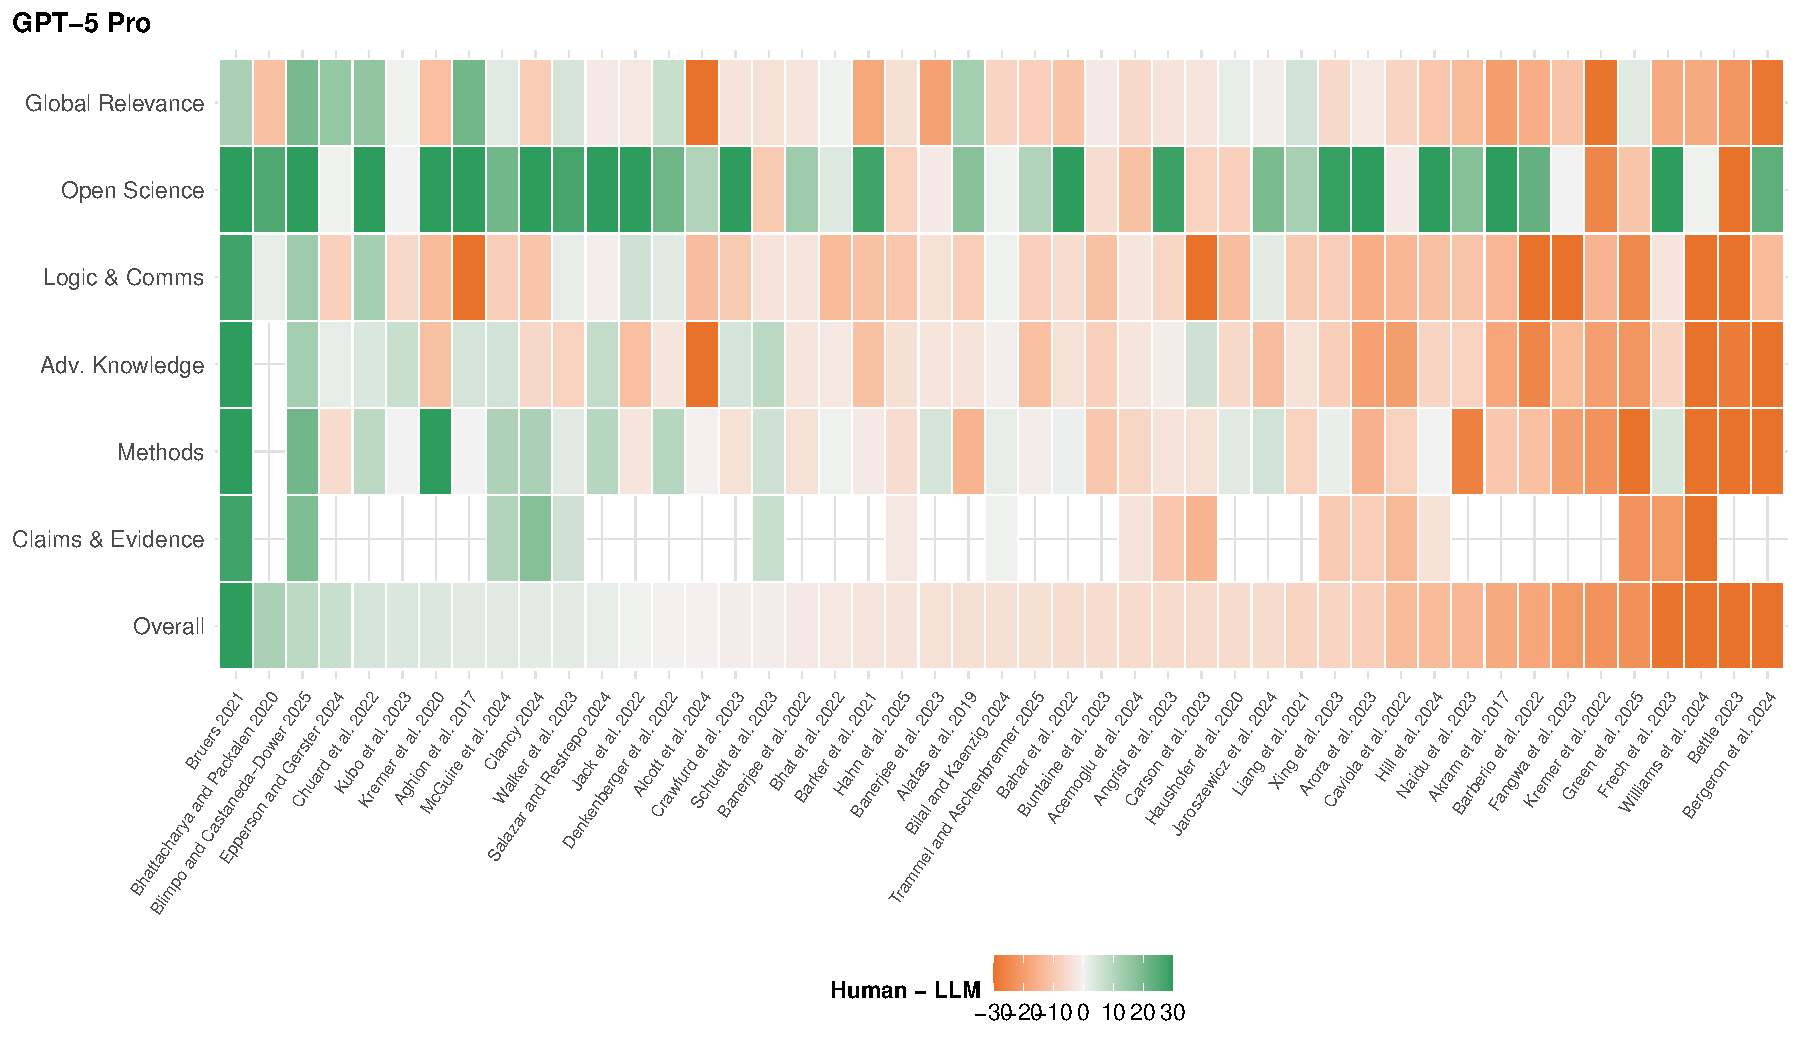
\includegraphics[keepaspectratio]{results_files/figure-pdf/fig-gap-heatmap-main-1.pdf}}

\end{figure}%

Rows with uniformly green or orange tiles indicate papers where humans
and the LLM disagree systematically across all criteria, not just on one
dimension. Columns with consistent colour suggest criteria-level biases.
Extended statistical analysis---including Krippendorff's alpha,
bootstrap confidence intervals, mutual information, tier correlations,
and top disagreement cases---is available in
\href{results_ratings.qmd}{Appendix A: Results Ratings}.

\bookmarksetup{startatroot}

\section{Discussion}\label{discussion}

Frontier LLMs achieve moderate-to-strong agreement with human expert
evaluators, approaching the ceiling set by inter-rater variability among
humans themselves. Correlations with human mean ratings are highest for
reasoning-capable models (GPT-5 Pro, Claude Opus 4.6), though even
lightweight models (GPT-4o-mini, Gemini 2.0 Flash) perform respectably
at a fraction of the cost. Central compression---the tendency for LLMs
to pull extreme ratings toward the middle of the scale---is the most
consistent pattern across all models, likely reflecting alignment
training that discourages confident extreme outputs. Qualitative
coverage varies widely across papers: on some, the LLM captures nearly
all consensus human concerns; on others, it misses key critiques or
raises issues absent from the expert consensus.

\textbf{Limitations.} Several caveats temper these conclusions. Our
sample comprises roughly 50 social-science papers specifically selected
by The Unjournal for evaluation, not a random draw from the research
literature; performance may differ in other fields or on less polished
manuscripts. Human evaluations are themselves a noisy reference signal
rather than ground truth, with substantial inter-rater variation that
caps achievable agreement. We cannot fully rule out knowledge
contamination: while we block extrinsic priors in the system prompt, the
models' training data may include fragments of these papers or related
discussions. Alignment training likely contributes to score inflation
and narrower credible intervals than humans provide. All LLM evaluations
are single-run; aggregating across multiple runs or temperature settings
could change the picture. Finally, the qualitative coverage and
precision metrics are themselves LLM-assessed (GPT-5.2 Pro as judge),
introducing a further layer of model dependence.

\textbf{Implications.} The cost structure is striking: lightweight
models deliver evaluations at under a cent per paper, while
reasoning-capable models cost several dollars---still orders of
magnitude cheaper than human expert review. This suggests a practical
tier structure in which cheap models could serve as rapid screening
tools and expensive reasoners could provide deeper assessment where
warranted. However, the qualitative gaps we observe---missed critiques,
generic issues, and central compression of ratings---argue against full
automation of peer review. AI evaluation appears most promising as a
supplement: providing fast structured feedback, flagging potential
concerns for human reviewers, and enabling systematic comparison across
large paper sets that would be infeasible with human effort alone.

\textbf{Future work.} Several extensions follow naturally from this
analysis. Content-swap bias tests following Pataranutaporn et al.
(\citeproc{ref-Pataranutaporn2025}{2025}) would reveal whether LLMs show
systematic biases based on author names or institutional affiliations. A
journal-outcome prediction horse-race would compare human and LLM tier
predictions against actual publication venues. Systematic prompt and
model comparisons, including agent-based approaches, could identify
configurations that reduce central compression or improve qualitative
coverage. Human enumerator validation---employing trained raters to
independently assess whether LLMs identify the same consensus
critiques---would ground the currently LLM-assessed coverage metrics.
Out-of-time validation using papers entering The Unjournal's pipeline
would eliminate contamination concerns entirely. Finally, hybrid
human-AI evaluation trials would test whether collaboration improves
evaluation quality beyond either alone.

\bookmarksetup{startatroot}

\section{Data and methods}\label{data-and-methods}

\small

We draw on two sources: human evaluations from
\href{https://unjournal.github.io/unjournaldata/index.html}{The
Unjournal's public evaluation data}, and LLM-generated evaluations
produced by prompting frontier models with The Unjournal's rubric and
requiring structured JSON output. We compare six models spanning three
providers: GPT-5 Pro, GPT-5.2 Pro, and GPT-4o-mini (OpenAI); Claude
Sonnet 4 and Claude Opus 4.6 (Anthropic); and Gemini 2.0 Flash (Google).
Each model returns a midpoint rating and 90\% credible interval for
every metric, enforced by a strict JSON Schema.

\subsection{Unjournal.org evaluations}\label{unjournal.org-evaluations}

We use The Unjournal's public data for a baseline comparison. At The
Unjournal each paper is typically evaluated (aka `reviewed') by two
expert evaluators\footnote{Occasionally they use 1 or 3 evaluators.} who
provide quantitative ratings on a 0--100 percentile scale for each of
seven criteria (with 90\% credible intervals),\footnote{See their
  guidelines
  \href{https://globalimpact.gitbook.io/the-unjournal-project-and-communication-space/policies-projects-evaluation-workflow/evaluation/guidelines-for-evaluators\#quantitative-metrics}{here};
  these criteria include ``Overall assessment'', ``Claims, strength and
  characterization of evidence'', ``Methods: Justification,
  reasonableness, validity, robustness'', ``Advancing knowledge and
  practice'', ``Logic and communication'', ``Open, collaborative,
  replicable science'', and ``Relevance to global priorities, usefulness
  for practitioners''} two ``journal tier'' ratings on a 0.0 - 5.0
scale,\footnote{``a normative judgment about `how well the research
  should publish'\,'' and ``a prediction about where the research will
  be published''} a written evaluation (resembling a referee report for
a journal), and identification and assessment of the paper's ``main
claim''. For our initial analysis, we extracted these human ratings and
aggregated them, taking the average score per criterion across
evaluators (and noting the range of individual scores).

All papers have completed The Unjournal's evaluation process (meaning
the authors received a full evaluation on the Unjournal platform, which
has been publicly posted at unjournal.pubpub.org). The sample includes
papers spanning 2017--2025 working papers in development economics,
growth, health policy, environmental economics, and related fields that
The Unjournal identified as high-impact. Each of these papers has
quantitative scores from at least one human evaluator, and many have
multiple (2-3) human ratings.

\subsection{LLM-based evaluation}\label{llm-based-evaluation}

Following The Unjournal's
\href{https://globalimpact.gitbook.io/the-unjournal-project-and-communication-space/policies-projects-evaluation-workflow/evaluation/guidelines-for-evaluators}{standard
guidelines for evaluators} and their
\href{https://coda.io/form/Unjournal-Evaluation-form-academic-stream-Coda-updated-version_dGjfMZ1yXME}{academic
evaluation form}, evaluators are asked to consider each paper along the
following dimensions: \textbf{claims \& evidence}, \textbf{methods},
\textbf{logic \& communication}, \textbf{open science}, \textbf{global
relevance}, and an \textbf{overall} assessment. Ratings are interpreted
as percentiles relative to serious recent work in the same area. For
each metric, evaluators are asked for the midpoint of their beliefs and
their 90\% credible interval, to communicate their uncertainty. For the
journal rankings measure, we ask both ``what journal ranking tier should
this work be published in? (0.0-5.0)'' and ``what journal ranking tier
will this work be published in? (0.0-5.0)'', with some further
explanation.The full prompt can be seen in the code below -- essentially
copied from the Unjournal's guidelines page.

We captured the versions of each paper that was evaluated by The
Unjournal's human evaluators, downloading from the links provided in The
Unjournal's Coda database.

We evaluate each paper by passing the PDF directly to the model and
requiring a strict, machine‑readable JSON output. This keeps the
assessment tied to the document the authors wrote. Direct ingestion
preserves tables, figures, equations, and sectioning, which ad‑hoc text
scraping can mangle. It also avoids silent trimming or segmentation
choices that would bias what the model sees.

\subsubsection{JSON Schema}\label{json-schema}

We enforce a strict JSON Schema for the output. The model must return
one object for each metric, including a midpoint rating and a 90\%
credible interval. This guarantees that every paper is scored on the
same fields with the same types and bounds. We request credible
intervals (as we do for human evaluators) to allow the model to
communicate its uncertainty rather than suggest false precision.

\subsubsection{System Prompt}\label{system-prompt}

The system prompt is built from modular sections and concatenated before
each API call. We instruct the model to act as an expert evaluator,
explicitly blocking the use of author reputation, publication venue, or
prior knowledge of the paper's reception. Before scoring, the prompt
requires a \textasciitilde1,000-word diagnostic summary (``think first,
score second'') that identifies methodological issues and guides
subsequent ratings.

Percentile ratings are anchored to the reference group ``all serious
research in the same area encountered in the last three years.'' The
prompt defines each of the seven criteria following The Unjournal's
\href{https://globalimpact.gitbook.io/the-unjournal-project-and-communication-space/policies-projects-evaluation-workflow/evaluation/guidelines-for-evaluators}{guidelines
for evaluators}, with emphasis on global priorities and practical
relevance over pure academic novelty.

The prompt also explains how to construct 90\% credible intervals (to
encourage calibrated uncertainty rather than artificially narrow
intervals), requests journal tier predictions on a 0--5 scale (providing
an external benchmark for papers that eventually publish), and includes
self-consistency checks requiring numeric scores to align with the
written assessment.

These sections are concatenated to form the complete system prompt:

The \texttt{evaluate\_paper} function uploads a PDF to the API and
submits a background job for evaluation:

Relying on GPT-5 Pro, we use a single‑step call with a reasoning model
that supports file input. One step avoids hand‑offs and summary loss
from a separate ``ingestion'' stage. The model reads the whole PDF and
produces the JSON defined above. We do not retrieve external sources or
cross‑paper material for these scores; the evaluation is anchored in the
manuscript itself.

The Python pipeline uploads each PDF once and caches the returned file
id keyed by path, size, and modification time. We submit one background
job per PDF to the OpenAI Responses API with ``high'' reasoning effort
and server‑side JSON‑Schema enforcement. Submissions record the response
id, model id, file id, status, and timestamps.

We then polls job status and, for each completed job, retrieve the raw
JSON object, and write the responses to disk.

\subsubsection{Multi-Model Evaluation}\label{multi-model-evaluation}

To compare model performance, we collect evaluations from multiple
providers. This allows us to assess whether different models exhibit
systematic biases or calibration differences.

For OpenAI models without reasoning (e.g., GPT-4o), we use a simpler
synchronous call:

Anthropic's API differs from OpenAI: PDFs are passed as base64-encoded
content, and calls are synchronous (no background jobs). We use Claude's
native PDF support.

Google's Gemini API supports PDF via file upload:

A unified runner collects evaluations from all providers:

\subsubsection{GPT-5.2 Pro Focal Run (with Key
Issues)}\label{gpt-5.2-pro-focal-run-with-key-issues}

This section evaluates 14 focal papers using GPT-5.2 Pro with an
extended schema that outputs a numbered list of key issues alongside the
standard metrics.

\subsubsection{Key Issues Comparison with Human
Critiques}\label{key-issues-comparison-with-human-critiques}

To validate how well the LLM identifies substantive issues, we compare
its \texttt{key\_issues} output against human expert critiques from The
Unjournal's Coda database. Human expert critiques provide a high-quality
reference standard for issue identification: they are produced by paid
domain experts and synthesized by evaluation managers, but remain noisy
and incomplete, so we treat them as a comparative signal rather than
ground truth.

The comparison proceeds in two stages: first, we extract and align the
data sources; then, optionally, we use an LLM to systematically assess
the degree of alignment between machine-generated and human-identified
issues.

The comparison pipeline uses a manually curated input and produces
structured outputs:

\textbf{Input:} - \textbf{\texttt{results/key\_issues\_comparison.md}}:
A manually curated markdown document pairing GPT-identified issues with
human expert critiques for each paper.

\textbf{Outputs:} -
\textbf{\texttt{results/key\_issues\_comparison.json}}: Parsed data in
JSON format for programmatic use. -
\textbf{\texttt{results/key\_issues\_comparison\_results.json}}:
LLM-assessed alignment metrics including coverage, precision, missed
issues, and overall ratings.

The coverage metric estimates what fraction of human-identified issues
the LLM captured; precision estimates what fraction of LLM issues are
genuinely relevant. Together with the qualitative ratings, these provide
a structured assessment of how well the LLM's issue identification
aligns with expert judgment.

\normalsize

\bookmarksetup{startatroot}

\section*{References}\label{references}
\addcontentsline{toc}{section}{References}

\markboth{References}{References}

\phantomsection\label{refs}
\begin{CSLReferences}{1}{0}
\bibitem[\citeproctext]{ref-aczel2021billion}
Aczel, Balazs, Barnabas Szaszi, and Alex O Holcombe, {``A billion-dollar
donation: Estimating the cost of researchers' time spent on peer
review,''} \emph{Research integrity and peer review}, 6 (2021), 1--8
(Springer).

\bibitem[\citeproctext]{ref-clancy2023returns}
Clancy, Matt, {``\href{https://arxiv.org/abs/2312.14289}{The returns to
science in the presence of technological risk},''} \emph{arXiv preprint
arXiv:2312.14289}, (2023).

\bibitem[\citeproctext]{ref-dycke2023}
Dycke, Nils, Ilia Kuznetsov, and Iryna Gurevych,
{``\href{https://aclanthology.org/2023.acl-long.277/}{{NLP}eer: A
unified resource for the computational study of peer review},''} in
\emph{Proceedings of the 61st annual meeting of the association for
computational linguistics (volume 1: Long papers)}, Anna Rogers, Jordan
Boyd-Graber, and Naoaki Okazaki, eds., 2023.

\bibitem[\citeproctext]{ref-eger2025}
Eger, Steffen, Yong Cao, Jennifer D'Souza, Andreas Geiger, Christian
Greisinger, Stephanie Gross, Yufang Hou, Brigitte Krenn, Anne Lauscher,
Yizhi Li, Chenghua Lin, Nafise Sadat Moosavi, Wei Zhao, and Tristan
Miller, {``\href{https://arxiv.org/abs/2502.05151}{Transforming science
with large language models: A survey on AI-assisted scientific
discovery, experimentation, content generation, and evaluation},''}
\emph{arXiv preprint arXiv:2505.05151}, (2025).

\bibitem[\citeproctext]{ref-korinek2025ai}
Korinek, Anton,
{``\href{https://papers.ssrn.com/sol3/papers.cfm?abstract_id=5455842}{AI
agents for economic research},''} \emph{SSRN Working Paper}, (2025).

\bibitem[\citeproctext]{ref-Luo2025}
Luo, Ziming, Zonglin Yang, Zexin Xu, Wei Yang, and Xinya Du,
{``\href{https://arxiv.org/abs/2501.04306}{LLM4SR: A survey on large
language models for scientific research},''} \emph{arXiv preprint
arXiv:2501.04306}, (2025).

\bibitem[\citeproctext]{ref-mitchener2025kosmos}
Mitchener, Ludovico, Ethan Yiu, and others,
{``\href{https://arxiv.org/abs/2511.02824}{Kosmos: An AI scientist for
autonomous discovery},''} \emph{arXiv preprint arXiv:2511.02824},
(2025).

\bibitem[\citeproctext]{ref-Pataranutaporn2025}
Pataranutaporn, Pat, Nattavudh Powdthavee, Chayapatr Achiwaranguprok,
and Pattie Maes,
{``\href{https://api.semanticscholar.org/CorpusID:277510314}{Can AI
solve the peer review crisis? A large scale cross model experiment of
LLMs' performance and biases in evaluating over 1000 economics
papers},''} 2025.

\bibitem[\citeproctext]{ref-son2025flaws}
Son, Jaeho, and others,
{``\href{https://arxiv.org/abs/2511.21843}{FLAWS: A benchmark for error
identification and localization in scientific papers},''} \emph{arXiv
preprint arXiv:2511.21843}, (2025).

\bibitem[\citeproctext]{ref-Zhang2025}
Zhang, Tianmai M, and Neil F Abernethy,
{``\href{https://arxiv.org/abs/2505.23824v2}{Reviewing scientific papers
for critical problems with reasoning LLMs: Baseline approaches and
automatic evaluation},''} \emph{arXiv preprint arXiv:2505.23824},
(2025).

\bibitem[\citeproctext]{ref-Zhang2025Replication}
Zhang, Yaohui, Haijing Zhang, Wenlong Ji, Tianyu Hua, Nick Haber,
Hancheng Cao, and Weixin Liang,
{``\href{https://arxiv.org/abs/2506.11343v1}{From replication to
redesign: Exploring pairwise comparisons for LLM-based peer review},''}
\emph{arXiv preprint arXiv:2506.11343}, (2025).

\end{CSLReferences}

\cleardoublepage
\phantomsection
\addcontentsline{toc}{part}{Appendices}
\appendix

\section{Results: Ratings}\label{results-ratings}

We compare quantitative ratings from 6 frontier LLMs (GPT-5 Pro, GPT-5.2
Pro, GPT-4o-mini, Claude Sonnet 4, Claude Opus 4.6, Gemini 2.0 Flash)
against human expert reviews from
\href{https://unjournal.pubpub.org}{The Unjournal}. 45 papers have both
human and LLM evaluations, enabling direct comparison across all seven
percentile criteria and two journal-tier predictions.

We submit each PDF through a single, schema-enforced API call. The
system prompt mirrors The Unjournal rubric, blocks extrinsic priors
(authors, venue, web context), and requires strict JSON: a
\textasciitilde1k-word diagnostic summary plus numeric midpoints and
90\% credible intervals for every metric.\footnote{0--100 percentiles
  relative to a reference group of \textasciitilde{}`all serious work
  you have read in this area in the last three years', overall (global
  quality/impact), claims\_evidence (claim clarity/support), methods
  (design/identification/robustness), advancing\_knowledge (contribution
  to field/practice), logic\_communication (internal consistency and
  exposition), open\_science (reproducibility, data/code availability),
  and global\_relevance (decision and priority usefulness). Journal
  tiers: (0--5, continuous) capture where the work should publish
  vs.~will publish.} Each numeric field carries a midpoint (model's 50\%
belief) and a 90\% credible interval; wide intervals indicate
acknowledged uncertainty.

\textbf{Cost and token usage.} Token costs are computed from
API-reported input/output tokens (GPT-5 Pro runs with \texttt{reasoning}
= high).

\begin{longtable}[]{@{}
  >{\raggedright\arraybackslash}p{(\linewidth - 12\tabcolsep) * \real{0.2099}}
  >{\raggedleft\arraybackslash}p{(\linewidth - 12\tabcolsep) * \real{0.0864}}
  >{\raggedleft\arraybackslash}p{(\linewidth - 12\tabcolsep) * \real{0.1235}}
  >{\raggedleft\arraybackslash}p{(\linewidth - 12\tabcolsep) * \real{0.1358}}
  >{\raggedleft\arraybackslash}p{(\linewidth - 12\tabcolsep) * \real{0.1728}}
  >{\raggedleft\arraybackslash}p{(\linewidth - 12\tabcolsep) * \real{0.1358}}
  >{\raggedleft\arraybackslash}p{(\linewidth - 12\tabcolsep) * \real{0.1358}}@{}}

\caption{\label{tbl-cost-overview}Token usage and estimated cost per
model}

\tabularnewline

\toprule\noalign{}
\begin{minipage}[b]{\linewidth}\raggedright
Model
\end{minipage} & \begin{minipage}[b]{\linewidth}\raggedleft
Papers
\end{minipage} & \begin{minipage}[b]{\linewidth}\raggedleft
Avg input
\end{minipage} & \begin{minipage}[b]{\linewidth}\raggedleft
Avg output
\end{minipage} & \begin{minipage}[b]{\linewidth}\raggedleft
Avg reasoning
\end{minipage} & \begin{minipage}[b]{\linewidth}\raggedleft
Total cost
\end{minipage} & \begin{minipage}[b]{\linewidth}\raggedleft
Cost/paper
\end{minipage} \\
\midrule\noalign{}
\endhead
\bottomrule\noalign{}
\endlastfoot
Claude Opus 4.6 & 45 & 116,930 & 1,509 & --- & \$84.02 & \$1.867 \\
GPT-5 Pro & 60 & 38,516 & 6,400 & 4,717 & \$57.71 & \$0.962 \\
GPT-5.2 Pro & 14 & 45,143 & 2,889 & 707 & \$11.91 & \$0.850 \\
Claude Sonnet 4 & 16 & 113,798 & 727 & --- & \$5.64 & \$0.352 \\
GPT-4o-mini & 60 & 71,581 & 470 & --- & \$0.66 & \$0.011 \\
Gemini 2.0 Flash & 60 & 18,084 & 1,024 & --- & \$0.10 & \$0.002 \\

\end{longtable}

Total cost across all 255 LLM evaluations: \textbf{\$160.03}.
Reasoning-capable models (GPT-5 Pro, GPT-5.2 Pro, Claude Opus 4.6) cost
substantially more per paper than their lighter counterparts
(GPT-4o-mini, Gemini 2.0 Flash), raising practical questions about
cost-quality trade-offs for deployment at scale.

\textbf{Agreement metrics.} We assess agreement using Pearson \emph{r}
(linear correlation), Spearman \emph{ρ} (rank-based, robust to
outliers), mean bias (LLM − Human; positive = LLM rates higher), and
RMSE/MAE (error magnitude).

\begin{longtable}[]{@{}lrrrrrr@{}}

\caption{\label{tbl-agreement}Agreement between each LLM and human mean
ratings (overall criterion)}

\tabularnewline

\toprule\noalign{}
Model & N & Pearson r & Spearman ρ & Mean bias & RMSE & MAE \\
\midrule\noalign{}
\endhead
\bottomrule\noalign{}
\endlastfoot
Claude Opus 4.6 & 33 & 0.567 & 0.477 & -7.6 & 17.2 & 12.4 \\
GPT-5 Pro & 45 & 0.342 & 0.517 & +6.4 & 15.4 & 10.3 \\
Gemini 2.0 Flash & 45 & 0.342 & 0.313 & -5.3 & 14.5 & 11.7 \\
GPT-5.2 Pro & 9 & 0.333 & 0.471 & -2.7 & 19.0 & 14.7 \\
GPT-4o-mini & 45 & 0.135 & 0.116 & +0.0 & 20.2 & 13.1 \\
Claude Sonnet 4 & 11 & 0.020 & 0.055 & +0.2 & 9.5 & 6.9 \\

\end{longtable}

Table~\ref{tbl-agreement} reports correlation and error metrics between
each LLM and the human mean overall rating. Positive mean bias indicates
the model rates papers higher than humans on average; negative bias
indicates harsher ratings. These correlations are bounded above by human
inter-rater noise---since the human ``mean'' is itself noisy, no model
can achieve a perfect correlation.

\textbf{Human baseline context.} To interpret human-LLM agreement, we
compare against human-human agreement as an upper bound. If human
evaluators only agree with each other at α = 0.5, expecting LLMs to
exceed that would be unrealistic. Table~\ref{tbl-human-baseline} shows
α\textsubscript{HH} (Krippendorff's alpha among human evaluators)
alongside α\textsubscript{HL} (between the human mean and each LLM).

\begin{longtable}[]{@{}
  >{\raggedright\arraybackslash}p{(\linewidth - 14\tabcolsep) * \real{0.1156}}
  >{\raggedleft\arraybackslash}p{(\linewidth - 14\tabcolsep) * \real{0.0340}}
  >{\raggedleft\arraybackslash}p{(\linewidth - 14\tabcolsep) * \real{0.1156}}
  >{\raggedleft\arraybackslash}p{(\linewidth - 14\tabcolsep) * \real{0.1293}}
  >{\raggedleft\arraybackslash}p{(\linewidth - 14\tabcolsep) * \real{0.1293}}
  >{\raggedleft\arraybackslash}p{(\linewidth - 14\tabcolsep) * \real{0.1565}}
  >{\raggedleft\arraybackslash}p{(\linewidth - 14\tabcolsep) * \real{0.1565}}
  >{\raggedleft\arraybackslash}p{(\linewidth - 14\tabcolsep) * \real{0.1633}}@{}}

\caption{\label{tbl-human-baseline}Human-human vs Human-LLM agreement by
criterion (Krippendorff's α)}

\tabularnewline

\toprule\noalign{}
\begin{minipage}[b]{\linewidth}\raggedright
Criterion
\end{minipage} & \begin{minipage}[b]{\linewidth}\raggedleft
α\_HH
\end{minipage} & \begin{minipage}[b]{\linewidth}\raggedleft
α\_HL (GPT-5 Pro)
\end{minipage} & \begin{minipage}[b]{\linewidth}\raggedleft
α\_HL (GPT-5.2 Pro)
\end{minipage} & \begin{minipage}[b]{\linewidth}\raggedleft
α\_HL (GPT-4o-mini)
\end{minipage} & \begin{minipage}[b]{\linewidth}\raggedleft
α\_HL (Claude Sonnet 4)
\end{minipage} & \begin{minipage}[b]{\linewidth}\raggedleft
α\_HL (Claude Opus 4.6)
\end{minipage} & \begin{minipage}[b]{\linewidth}\raggedleft
α\_HL (Gemini 2.0 Flash)
\end{minipage} \\
\midrule\noalign{}
\endhead
\bottomrule\noalign{}
\endlastfoot
Overall & 0.55 & 0.25 & 0.36 & 0.14 & 0.06 & 0.47 & 0.25 \\
Claims & 0.42 & 0.20 & 0.26 & 0.19 & 0.21 & 0.26 & 0.18 \\
Methods & 0.54 & 0.29 & 0.07 & 0.03 & -0.22 & 0.39 & 0.16 \\
Adv. Knowledge & 0.20 & 0.18 & 0.20 & 0.13 & 0.06 & 0.32 & 0.07 \\
Logic \& Comms & 0.33 & -0.04 & -0.19 & -0.00 & 0.26 & 0.09 & -0.03 \\
Open Science & 0.03 & -0.06 & -0.61 & -0.16 & 0.25 & -0.18 & 0.03 \\
Global Relevance & 0.33 & 0.25 & 0.51 & 0.04 & 0.06 & 0.18 & 0.17 \\

\end{longtable}

Where α\textsubscript{HL} approaches α\textsubscript{HH}, the LLM is
performing at or near the ceiling set by human inter-rater variability.
Criteria where α\textsubscript{HH} is already low (indicating genuine
evaluator disagreement) naturally cap how well any model can do.
Extended agreement analysis---including CI coverage, bootstrap
confidence intervals, mutual information, and per-criterion
correlations---is available in the supplementary material.

\textbf{Criteria-level patterns.} Figure~\ref{fig-criteria-heatmap}
displays the mean rating each evaluator type assigns across the seven
criteria. Criteria where all models and humans converge (similar colour
intensity) suggest robust agreement on that dimension; criteria with
divergent columns indicate systematic differences in how humans and LLMs
weigh that aspect of quality.

\begin{figure}

\caption{\label{fig-criteria-heatmap}Mean rating by model and criterion}

\pandocbounded{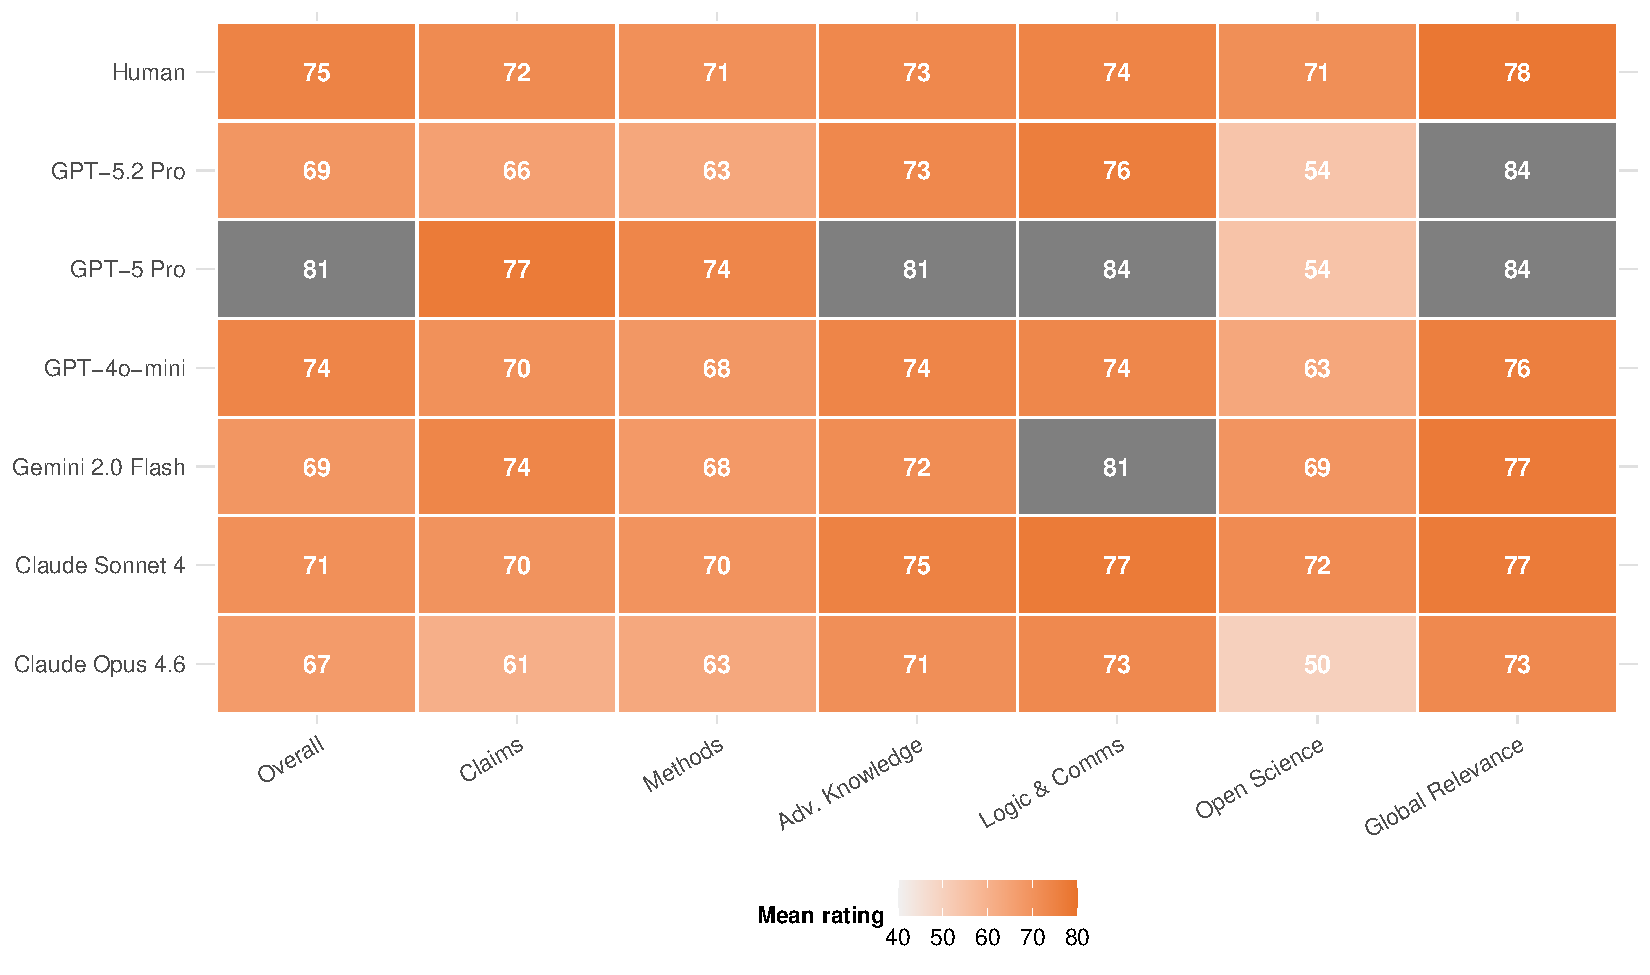
\includegraphics[keepaspectratio]{results_ratings_files/figure-pdf/fig-criteria-heatmap-1.pdf}}

\end{figure}%

For per-paper scatter plots, rank comparisons, and the gap heatmap
showing Human − LLM differences by paper and criterion, see the
\hyperref[results]{main Results chapter}. Extended reasoning traces are
available in \href{appendix_llm_traces.qmd}{Appendix C: LLM Traces}.

\section{Results: Critiques \& Key
Issues}\label{results-critiques-key-issues}

This chapter reports preliminary results from comparing LLM-identified
key issues against human expert critiques. The analysis uses LLM-based
assessment (GPT-5.2 Pro as judge) to measure coverage and precision;
human validation of these alignment scores is underway.

\begin{tcolorbox}[enhanced jigsaw, opacityback=0, leftrule=.75mm, titlerule=0mm, toptitle=1mm, opacitybacktitle=0.6, colframe=quarto-callout-warning-color-frame, left=2mm, arc=.35mm, coltitle=black, breakable, bottomrule=.15mm, bottomtitle=1mm, colback=white, colbacktitle=quarto-callout-warning-color!10!white, toprule=.15mm, title=\textcolor{quarto-callout-warning-color}{\faExclamationTriangle}\hspace{0.5em}{Warning}, rightrule=.15mm]

This section is under active development. Coverage and precision metrics
below are LLM-assessed; manual annotation is in progress.

\end{tcolorbox}

\textbf{Data sources.} We compare GPT-5.2 Pro key issues (structured
output from the focal evaluation run, January 2026) against human expert
critiques curated from The Unjournal's internal tracking database, where
evaluation managers synthesize evaluator feedback using severity labels
(``Necessary'', ``Optional but important'', ``Unsure'').

We matched \textbf{14 papers} with both GPT-5.2 Pro key issues and human
expert critiques.

\textbf{LLM-based assessment.} The comparison was assessed using GPT-5.2
Pro, which evaluated coverage (what proportion of human concerns GPT
identified) and precision (whether GPT issues are substantive).

\begin{itemize}
\tightlist
\item
  \textbf{Coverage}: Proportion of \emph{consensus} human issues that
  have any LLM match (match quality \textgreater= 30\%)
\item
  \textbf{Weighted Coverage}: Mean match quality across all human issues
  (treating unmatched issues as 0\%)
\item
  \textbf{Precision}: Proportion of LLM issues that match a human
  concern
\end{itemize}

\begin{tcolorbox}[enhanced jigsaw, opacityback=0, leftrule=.75mm, titlerule=0mm, toptitle=1mm, opacitybacktitle=0.6, colframe=quarto-callout-note-color-frame, left=2mm, arc=.35mm, coltitle=black, breakable, bottomrule=.15mm, bottomtitle=1mm, colback=white, colbacktitle=quarto-callout-note-color!10!white, toprule=.15mm, title=\textcolor{quarto-callout-note-color}{\faInfo}\hspace{0.5em}{Caveat on Precision}, rightrule=.15mm]

``Precision'' only reflects whether LLM issues match the
\emph{consensus} human issues curated in Coda---those prioritized by
evaluation managers as the most important concerns. Many LLM-identified
issues may have been noted by one or more individual human evaluators
but were not included in this curated set. A low precision score does
not necessarily mean the LLM raised irrelevant concerns; it may simply
reflect issues that weren't prioritized in the consensus summary.

\end{tcolorbox}

\begin{tcolorbox}[enhanced jigsaw, opacityback=0, leftrule=.75mm, titlerule=0mm, toptitle=1mm, opacitybacktitle=0.6, colframe=quarto-callout-note-color-frame, left=2mm, arc=.35mm, coltitle=black, breakable, bottomrule=.15mm, bottomtitle=1mm, colback=white, colbacktitle=quarto-callout-note-color!10!white, toprule=.15mm, title=\textcolor{quarto-callout-note-color}{\faInfo}\hspace{0.5em}{Interpretation Guide}, rightrule=.15mm]

\begin{itemize}
\tightlist
\item
  \textbf{Coverage}: Percentage of human-identified issues that GPT also
  captured (in some form). Higher = GPT missed fewer human concerns.
\item
  \textbf{Precision}: Percentage of GPT issues that are substantive
  rather than generic or spurious. Higher = GPT's critiques are more
  targeted.
\item
  \textbf{Overall Rating}: Qualitative assessment
  (Excellent/Good/Moderate/Poor) based on both coverage and precision
  metrics.
\end{itemize}

\end{tcolorbox}

The coverage-precision figure above shows substantial variation across
papers: some papers achieve high coverage and precision, while others
show the LLM missing key human concerns or raising issues not in the
expert consensus. Paper-by-paper comparisons with matched issue pairs,
structural difference tables, and the manual annotation tool are
available in the
\href{https://llm-uj-research-eval.netlify.app/results_critiques.html}{full
online version}.

\section{Supplementary Material}\label{supplementary-material}

\subsection{Related Work}\label{sec-related-work}

\subsubsection{AI practical research
applications}\label{ai-practical-research-applications}

Luo et al. (\citeproc{ref-Luo2025}{2025}) survey LLM roles from idea
generation to peer review, including experiment planning and automated
scientific writing. They highlight opportunities (productivity, coverage
of long documents) alongside governance needs (provenance, detection of
LLM-generated content, standardizing tooling) and call for reliable
evaluation frameworks.

Korinek (\citeproc{ref-korinek2025ai}{2025}) considers the specific
potential for using AI in economic research, offering ``working examples
and step-by-step code'' to help economists use agents for literature
reviews, econometric code, fetching and analyzing economic data, and
coordinate complex research workflows. He advocates economists using AI
tools to boost productivity and ``to understand {[}these tools'{]}
capabilities and limitations.'' He calls for human researcher oversight
``to ensure {[}these tools{]} pursue the right objectives and maintain
research integrity''. He outlines a range of current limitations and
open questions (outlined
\href{https://docs.google.com/document/d/1CVNnG6Jw3gr1sbI9Z_vIIJ1BI9O-8-Eev6D2j22vaeg/edit?tab=t.0\#heading=h.9pcc2azfjlro}{here}),
including hallucinations, mistakes compounding through multi-agent
workflows and ``brittleness to small variations in prompts''. At the
higher level, he argues ``the questions that will matter most---what
problems deserve investigation, how should we evaluate trade-offs, what
constitutes progress---will remain irreducibly human.''

Mitchener, Yiu, et al. (\citeproc{ref-mitchener2025kosmos}{2025})
present Kosmos, ``an AI scientist for autonomous discovery''. However,
evaluations reveal important limitations: Kosmos was found to be only
57\% accurate in statements that required interpretation of results, and
``identifying valuable discoveries Kosmos made is a time-intensive
process that relies on human scientists with significant domain
expertise.''

\subsubsection{AI peer review, error detection, and research
evaluation}\label{ai-peer-review-error-detection-and-research-evaluation}

Son et al. (\citeproc{ref-son2025flaws}{2025}) evaluates LLMs on 83
papers paired with 91 confirmed significant scientific errors. Their
strongest (OpenAI o3) model identified only 21.1\% of these errors, with
only 6.1\% precision---domain experts found most false positives were
hallucinations or student-level misconceptions.

Eger et al. (\citeproc{ref-eger2025}{2025}) provide a broad review of
LLMs in science and a focused discussion of AI-assisted peer review.
They argue: (i) peer-review data is scarce and concentrated in
CS/OpenReview venues; (ii) targeted assistance that preserves human
autonomy is preferable to end-to-end reviewing; and (iii) ethics and
governance (bias, provenance, detection of AI-generated text) are
first-class constraints.

Dycke, Kuznetsov, and Gurevych (\citeproc{ref-dycke2023}{2023}) present
NLPEER, a ``multidomain corpus'' of more than 5000 papers and 11k review
reports from 2012 to 2022 from five different venues.

Zhang and Abernethy (\citeproc{ref-Zhang2025}{2025}) propose deploying
LLMs as quality checkers to surface critical problems instead of
generating full narrative reviews. Using papers from WITHDRARXIV and an
automatic evaluation framework that leverages ``LLM-as-judge,'' they
find the best performance from top reasoning models but still recommend
human oversight.

Pataranutaporn et al. (\citeproc{ref-Pataranutaporn2025}{2025}) asked
four nearly state-of-the-art LLM models to consider 1220 unique papers
drawn from 110 economics journals excluded from the training data of
current LLMs. They find general alignment between LLM ratings and RePEC
journal rankings, mixed results on detecting AI-generated papers, and
evidence that LLMs show biases towards named high-prestige male authors
and elite institutions.

Zhang et al. (\citeproc{ref-Zhang2025Replication}{2025}) use AI
conference paper data and LLM agents for pairwise manuscript
comparisons, finding this approach outperforms traditional rating-based
methods for identifying high-impact papers by citation metrics, though
with some evidence of biases favoring established research institutions.

\subsubsection{AI research taste and potential to guide
research}\label{ai-research-taste-and-potential-to-guide-research}

A key motivation for this work stems from broader claims about AI's
potential to accelerate scientific discovery. If AI systems are to
contribute meaningfully to research---not just as tools but as
evaluators and potential collaborators---we need to understand their
``taste'': what they value, what they miss, and whether their priorities
align with human expert judgment and real-world research impact. This
connects to broader debates about the returns to science in the presence
of technological risk (\citeproc{ref-clancy2023returns}{Clancy 2023}).

\subsection{Extended Rating Analysis}\label{extended-rating-analysis}

The main text reports six core exhibits: cost overview, human-vs-LLM
scatter plot, agreement metrics, human baseline (Krippendorff's alpha),
criteria-level heatmap, and gap heatmap. The following extended analyses
are preserved in the project's git history and available in earlier
rendered versions:

\begin{itemize}
\tightlist
\item
  \textbf{Krippendorff's alpha by criterion}: Inter-rater agreement
  treating human mean and each LLM as separate raters
\item
  \textbf{CI coverage analysis}: Share of human mean ratings falling
  within LLM 90\% credible intervals
\item
  \textbf{Bootstrap 95\% CIs}: Nonparametric confidence intervals for
  Pearson correlations
\item
  \textbf{Mutual information}: Information-theoretic measure of
  human-LLM rating dependence
\item
  \textbf{Per-criterion correlations}: Pearson and Spearman by
  evaluation criterion and model
\item
  \textbf{Tier correlation dumbbell plot}: How criteria predict journal
  tier judgments for humans vs.~LLMs
\item
  \textbf{Top disagreement cases}: Papers with largest human-LLM rating
  differences
\item
  \textbf{Prompt comparison}: Legacy vs.~updated GPT-5 Pro prompt effect
  on ratings
\end{itemize}

\subsection{Extended Critique
Analysis}\label{extended-critique-analysis}

The main text reports coverage-precision scatter and summary statistics.
The following extended analyses are available in the
\href{https://llm-uj-research-eval.netlify.app/results_critiques.html}{full
online version}:

\begin{itemize}
\tightlist
\item
  \textbf{Paper-by-paper issue comparisons}: Interactive collapsible
  panels showing matched issue pairs, unmatched human/LLM issues, and
  detailed discussion for each paper
\item
  \textbf{Aggregate statistics}: Total issue counts by severity, human
  vs.~LLM issue distributions
\item
  \textbf{Observable structural differences}: Format, structure,
  attribution, and length comparisons
\item
  \textbf{Manual annotation tool}: Browser-based UI for systematic
  concordance labeling
\end{itemize}

\begin{center}\rule{0.5\linewidth}{0.5pt}\end{center}

\emph{The per-paper LLM evaluation traces below are only available in
the
\href{https://llm-uj-research-eval.netlify.app/appendix_llm_traces.html}{online
HTML version}.}




\end{document}
